\documentclass{article}
\usepackage{graphicx}
\usepackage{geometry}
\usepackage{amsmath,mathpazo}
\usepackage{amssymb}
\usepackage{mathtools}
\usepackage{commath}
\usepackage{enumitem}
\usepackage{listings}
\usepackage{hyperref}

\geometry{
  top=20mm,
}
\newcommand{\boldvec}[1]{\boldsymbol{\vec{\textbf{#1}}}}
\newcommand{\capvec}[1]{\boldsymbol{\hat{\textbf{#1}}}}
\newcommand{\bld}[1]{\textbf{#1}}
\newcommand{\ital}[1]{\textit{#1}}
\newcommand{\italb}[1]{\textbf{\textit{{#1}}}}
\begin{document}

\title{Introduction to Parallel \&
Distributed Programming\\COL380 -Programming Assignment 1}
\author{Ankesh Gupta\\2015CS10435}

\date{}
\maketitle

\section*{Parallel Convex Hull}

\bld{Data Structures and Design Decisions}
\begin{enumerate}
\item The algorithm was adapted from \href{https://en.wikipedia.org/wiki/Quickhull}{\ital{Quickhull Algorithm}} algorithm on $Wikipedia$.
\item Its uses a \ital{divide and conquer} to locate mandatory hull points, and then discard points lying on the inside of enclosing rectangle.
\item The program has been attempted to parallize by making the recursive $quickhull$ call being run on an independent thread.
\item Also, call to recursive function inside $pragma$ construct was made \ital{non blocking/no wait}, so as to allow other threads to work in parallel.
\item Data Structures used were vectors, a \ital{dynamic-array}. The reason was because it is mutable and doesnt require size declaration as beginning.
\item To limit the \ital{number of threads}, a global counter was maintained, shared by all threads, which tracked how many threads are available.
\item Each time a thread get created/destroyed, an access is made to the variable(mentioned above), which according to availability, may either accept/reject request.
\item If threads are not available, the remaining program becomes sequential.
\end{enumerate}

\bld{Analyzing Graphs}
\begin{enumerate}
	\item The efficiency curve follows a similar trend as it was in prefix sum case: Decreases with increase in thread(for any problem size).
	\item Speedup curve is different. Never is the speedup of parallel implementation $>$ 1.
	\item This reflects that the algorithm is indeed suffering from large serial component, which can't be parallelised.
	\item One of the major time consuming operation is generation of the \ital{candidate hull points} from the image.
	\item Passing vector references would add on to speedup of the program.
	\item But, one trend persists. With increase in problem size, speedup acheived showed an increasing trend(though less than 1). This is consistent with \italb{Gustafson's Law}.
\end{enumerate}
% \item For problem size of n and p resources, partial prefix sum is calculated in $O(n/p)$ time and $O(n)$ work.
% \item The p partial sums  are then combined using the $wiki$ algorithm mentioned in point 1 in $O(\log{p})$ time and $O(p)$ .
% \item Again, those p partial sums are reflected back on original array in $O(n/p)$ time and $O(n)$ work.
% \item For all parts, arrays and vectors were used which support fast random access.
% \item The main logic to perform point 4 was to exploit \ital{cache locality}.
% \item There was no need to take care about \italb{false sharing} as because in calculating partial sums, question of false sharing is irrelevant as threads work on different arrays chunks.
% \item In combining partial prefix sum's, array accesses quite random($i$ and $2^i$) and so preventing false sharing is of little use.
% \end{enumerate}  

% \bld{Analyzing Figures}
% \begin{enumerate}
% 	\item The experiments were performed on a 6 core Processor.
% 	\item Amongst the experiments performed, graph for $speedup$ showed similar trends. The best speedup was from graph appears around $(4-5)$.
% 	\item Speedup declines because of increased overhead when threads are greater than cores.
% 	\item Speedup increases with increase in problem size, as serial component remains same(\italb{Gustafson's Law}). Also, speedup appears to peak around 1.5 for a given problem size(\italb{Amdahl's Law}).
% 	\item Efficiency graph shows a consistent trend. It decreases with increasing processor.
% 	\item The above phenomenon was intuitive because single thread programs are most efficient.
% \end{enumerate}
\begin{figure}[h]
\vspace*{-2cm}
\centering
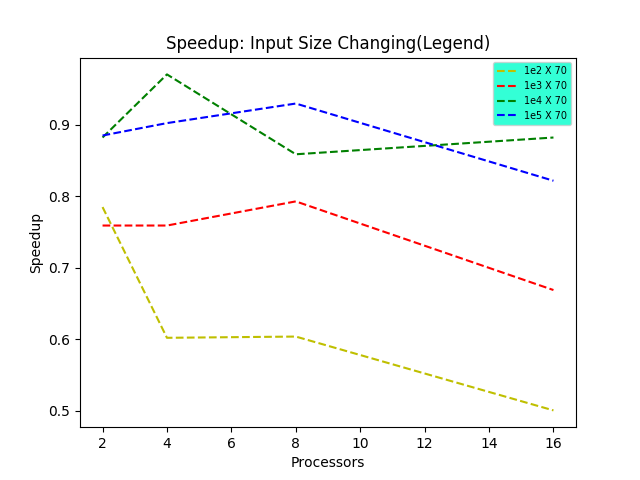
\includegraphics[scale=0.9]{Part2S.png}
\caption{Speedup vs Processors for Varying input}
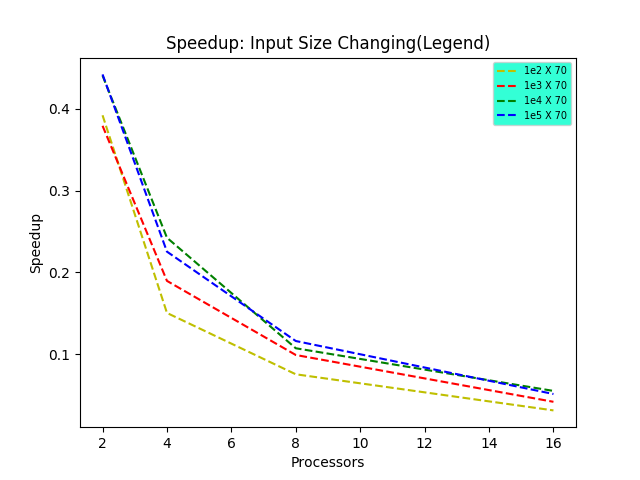
\includegraphics[scale=0.9]{Part2E.png}
\caption{Efficiency vs Processors for Varying input}
\end{figure}

\end{document}
